\documentclass[11pt,a4paper]{article}
\usepackage[margin=0.75in]{geometry}
\usepackage{graphicx}
\usepackage{booktabs}
\usepackage{hyperref}
\usepackage{amsmath}
\usepackage{enumitem}
\usepackage{float}
\usepackage{caption}
\usepackage{multicol}

\title{\textbf{CSL 7640: Natural Language Understanding}\\Programming Assignment 2}
\author{Sunny Singh\\IIT Jodhpur}
\date{March 2026}

\begin{document}
\maketitle

% =============================================
% PROBLEM 1
% =============================================
\section{Problem 1: Semantic Analysis using Word2Vec}

\subsection{Task 1: Dataset Preparation}

\subsubsection{Corpus Curation}
We scraped textual data from \textbf{10 IIT Jodhpur web pages} (Homepage, Introduction, History, Office of Academics, BTech Programs, CSE Department, ME UG Program, R\&D, PhD Programs, CSE Faculty) and extracted text from the \textbf{Academic Regulations PDF}.

\subsubsection{Preprocessing Steps}
\begin{enumerate}[noitemsep]
    \item Scraped web pages using \texttt{requests} + \texttt{BeautifulSoup}; removed HTML boilerplate tags.
    \item Extracted PDF text using \texttt{PyPDF2}.
    \item Removed boilerplate: URLs, emails, copyright notices, phone numbers, non-ASCII characters.
    \item Sentence tokenization using NLTK \texttt{sent\_tokenize}.
    \item Word tokenization using NLTK \texttt{word\_tokenize}.
    \item Lowercased all tokens.
    \item Removed non-alphabetic tokens and tokens with length $<$ 2.
    \item Saved cleaned corpus (one sentence per line).
\end{enumerate}

\subsubsection{Corpus Statistics}
\begin{itemize}[noitemsep]
    \item \textbf{Corpus size:} 0.11 MB (cleaned), 0.18 MB (raw)
    \item \textbf{Documents:} 10 (9 web pages + 1 PDF)
    \item \textbf{Total tokens:} 17,523
    \item \textbf{Vocabulary size:} 2,263
\end{itemize}

\noindent\textbf{Top-10 words (frequency-wise):}\\
the (1344), of (878), and (455), to (433), for (406), in (387), be (292), student (240), or (184), will (180)

\subsubsection{Word Cloud}
\begin{figure}[H]
    \centering
    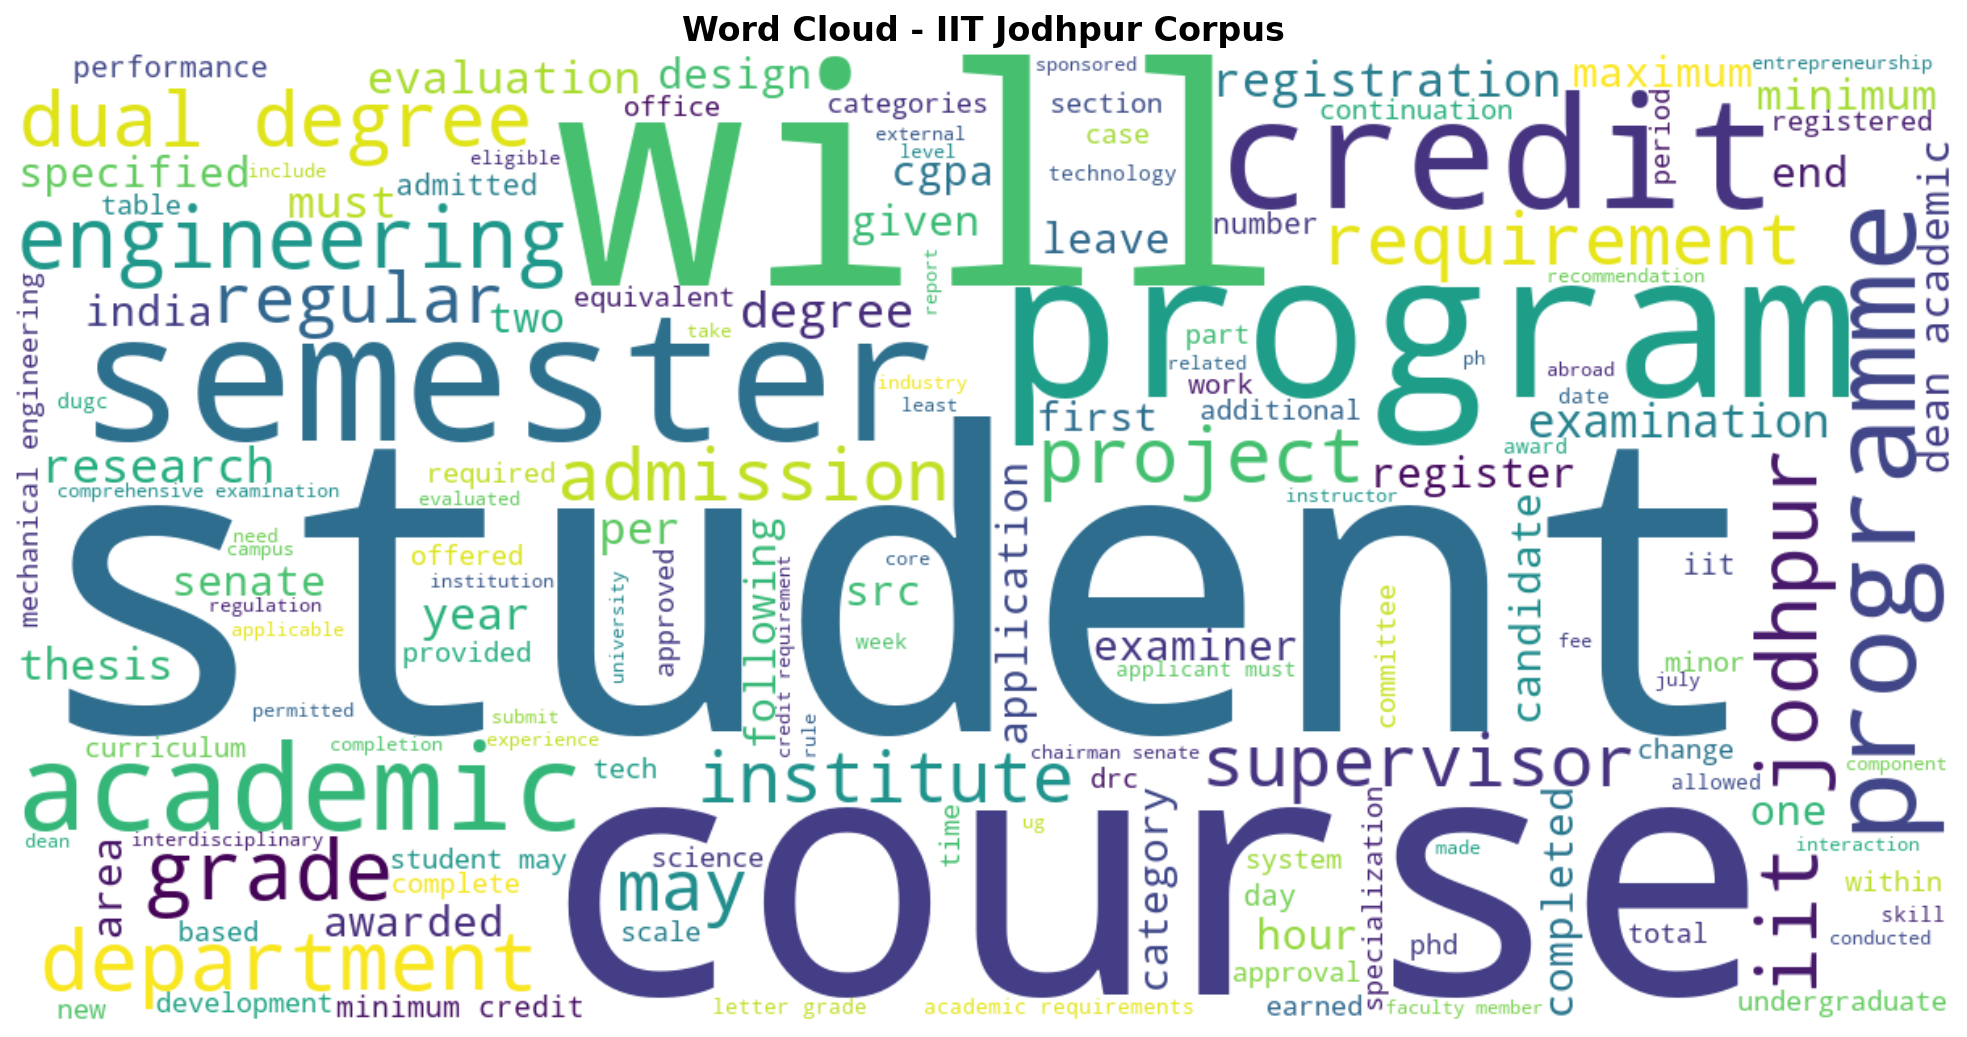
\includegraphics[width=0.65\textwidth]{Problem1/outputs/wordcloud.png}
    \caption{Word Cloud of the IIT Jodhpur Corpus}
\end{figure}

% ----- Task 2 -----
\subsection{Task 2: Word2Vec Training}

We trained both \textbf{CBOW} and \textbf{Skip-gram} models with hyperparameter experiments varying embedding dimension $\{50, 100, 200\}$, window size $\{3, 5, 7\}$, and negative samples $\{5, 10, 15\}$. Models were trained for 20 epochs with \texttt{min\_count=2}.

\begin{table}[H]
\centering
\caption{Selected Hyperparameter Experiment Results}
\small
\begin{tabular}{lccccr}
\toprule
\textbf{Model} & \textbf{Dim} & \textbf{Window} & \textbf{Neg} & \textbf{AvgSim} & \textbf{Vocab} \\
\midrule
CBOW      & 50  & 5 & 10 & 0.9711 & 1267 \\
Skip-gram & 50  & 5 & 10 & 0.7629 & 1267 \\
CBOW      & 100 & 5 & 10 & 0.9803 & 1267 \\
Skip-gram & 100 & 5 & 10 & 0.7691 & 1267 \\
CBOW      & 200 & 5 & 10 & 0.9875 & 1267 \\
Skip-gram & 200 & 5 & 10 & 0.7891 & 1267 \\
\bottomrule
\end{tabular}
\end{table}

Best models (dim=100, window=5, neg=10) were saved for subsequent analysis.

% ----- Task 3 -----
\subsection{Task 3: Semantic Analysis}

\subsubsection{Nearest Neighbors}

\begin{table}[H]
\centering
\caption{Top-3 Nearest Neighbors -- CBOW vs Skip-gram}
\small
\begin{tabular}{lll}
\toprule
\textbf{Word} & \textbf{CBOW} & \textbf{Skip-gram} \\
\midrule
research & development (0.82), proposal (0.79) & proposal (0.71), projects (0.65) \\
student  & registration (0.81), course (0.78) & candidacy (0.68), attendance (0.64) \\
phd      & eligibility (0.84), mtech (0.83) & mtech (0.72), enrolled (0.67) \\
exam     & seminar (0.80), attend (0.76) & scholars (0.69), conferences (0.66) \\
\bottomrule
\end{tabular}
\end{table}

\noindent CBOW produces higher similarity scores (0.78--0.84) due to averaging context words, while Skip-gram shows more varied scores (0.64--0.72) capturing finer semantic distinctions.

\subsubsection{Analogy Experiments}

\begin{itemize}[noitemsep]
    \item \textbf{UG : undergraduate :: PG : ?} $\rightarrow$ \textbf{postgraduate} (sim: 0.9943, CBOW)
    \item \textbf{student : exam :: professor : ?} $\rightarrow$ electrical (0.98), university (0.97)
    \item \textbf{department : faculty :: lab : ?} $\rightarrow$ on (0.97), leave (0.96)
\end{itemize}

The first analogy successfully captures the academic degree hierarchy. The other analogies are less precise due to the small corpus size.

% ----- Task 4 -----
\subsection{Task 4: Visualization}

\begin{figure}[H]
    \centering
    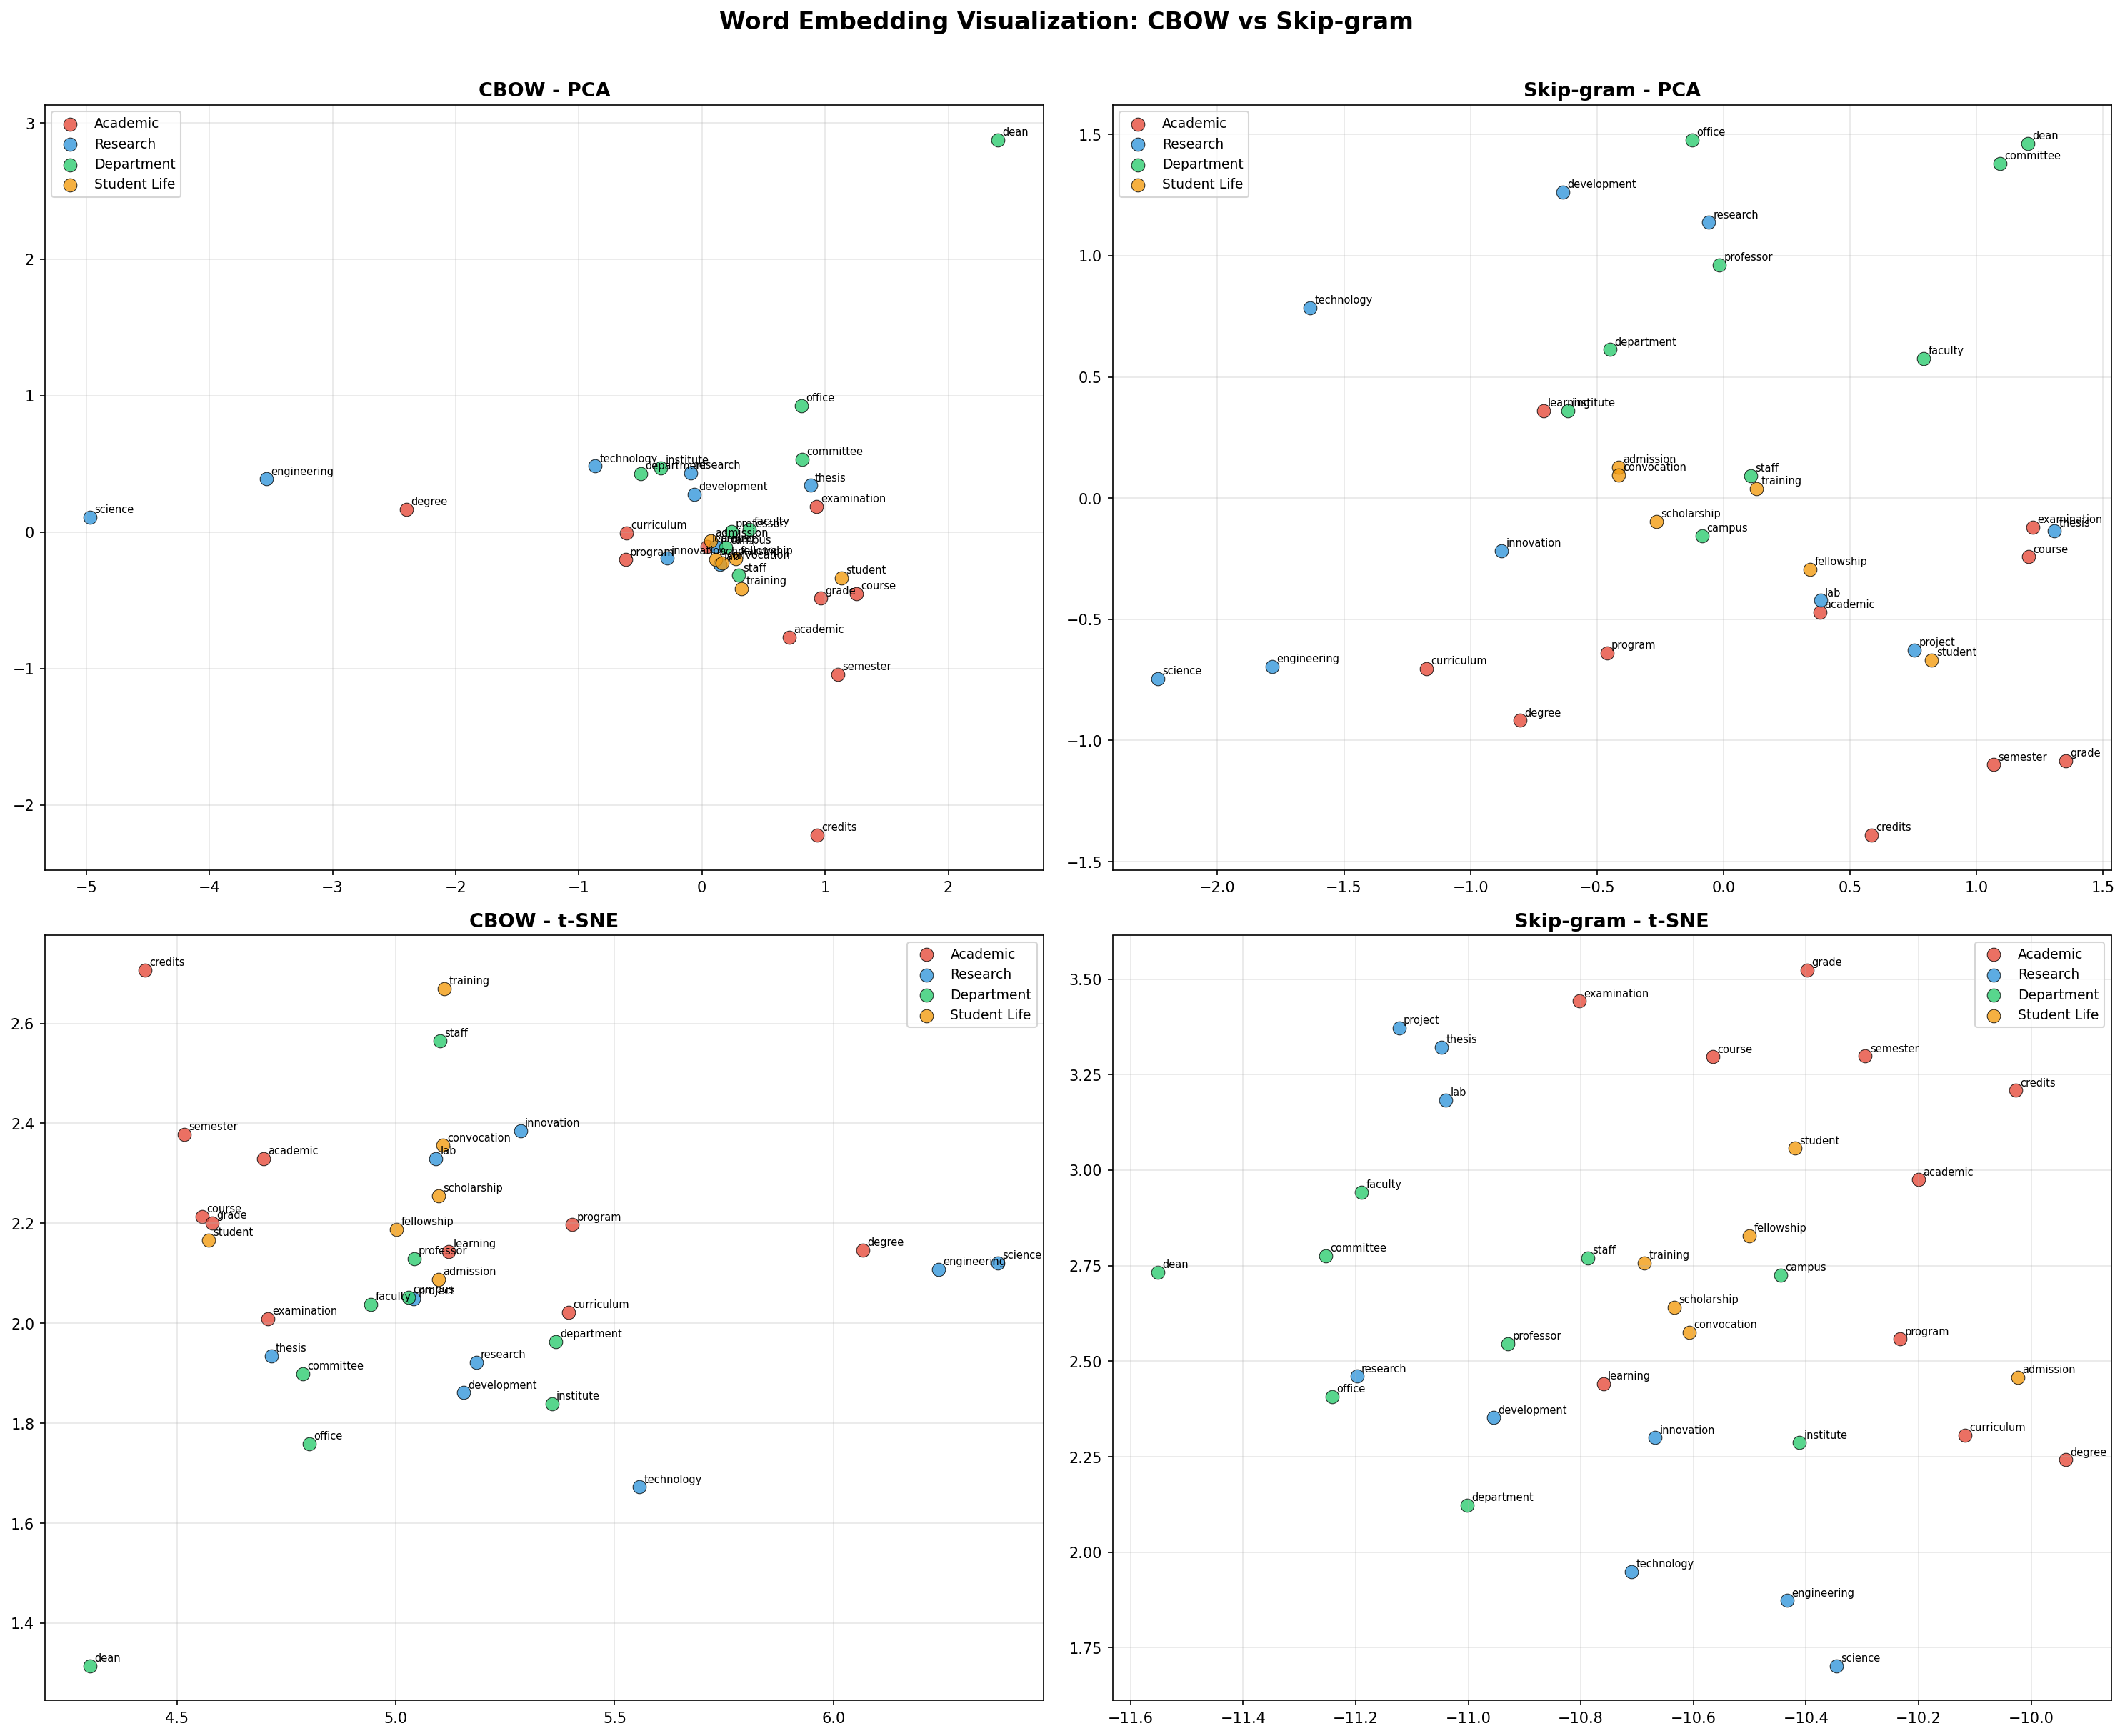
\includegraphics[width=0.85\textwidth]{Problem1/outputs/comparison_plot.png}
    \caption{CBOW vs Skip-gram: PCA and t-SNE Visualizations}
\end{figure}

Academic, research, department, and student-life word clusters show meaningful grouping in both models. Skip-gram produces more dispersed but semantically informative clusters, while CBOW yields tighter clusters for frequent words.

% =============================================
% PROBLEM 2
% =============================================
\section{Problem 2: Character-Level Name Generation}

\subsection{Task 1--3: Model Architectures}

We implemented three models for character-level Indian name generation using a dataset of 1,000 curated Indian names. All models use embedding dim=32, hidden size=128, 1 layer, trained for 100 epochs with lr=0.003 and batch size=64.

\begin{table}[H]
\centering
\caption{Model Architecture Comparison}
\begin{tabular}{lccc}
\toprule
\textbf{Model} & \textbf{Parameters} & \textbf{Size (MB)} & \textbf{Description} \\
\midrule
Vanilla RNN    & 25,244  & 0.10 & Single-layer RNN with tanh \\
BLSTM          & 173,980 & 0.67 & Bidirectional LSTM \\
Attention RNN  & 124,188 & 0.48 & LSTM + Causal Attention \\
\bottomrule
\end{tabular}
\end{table}

\subsection{Training Loss}

\begin{figure}[H]
    \centering
    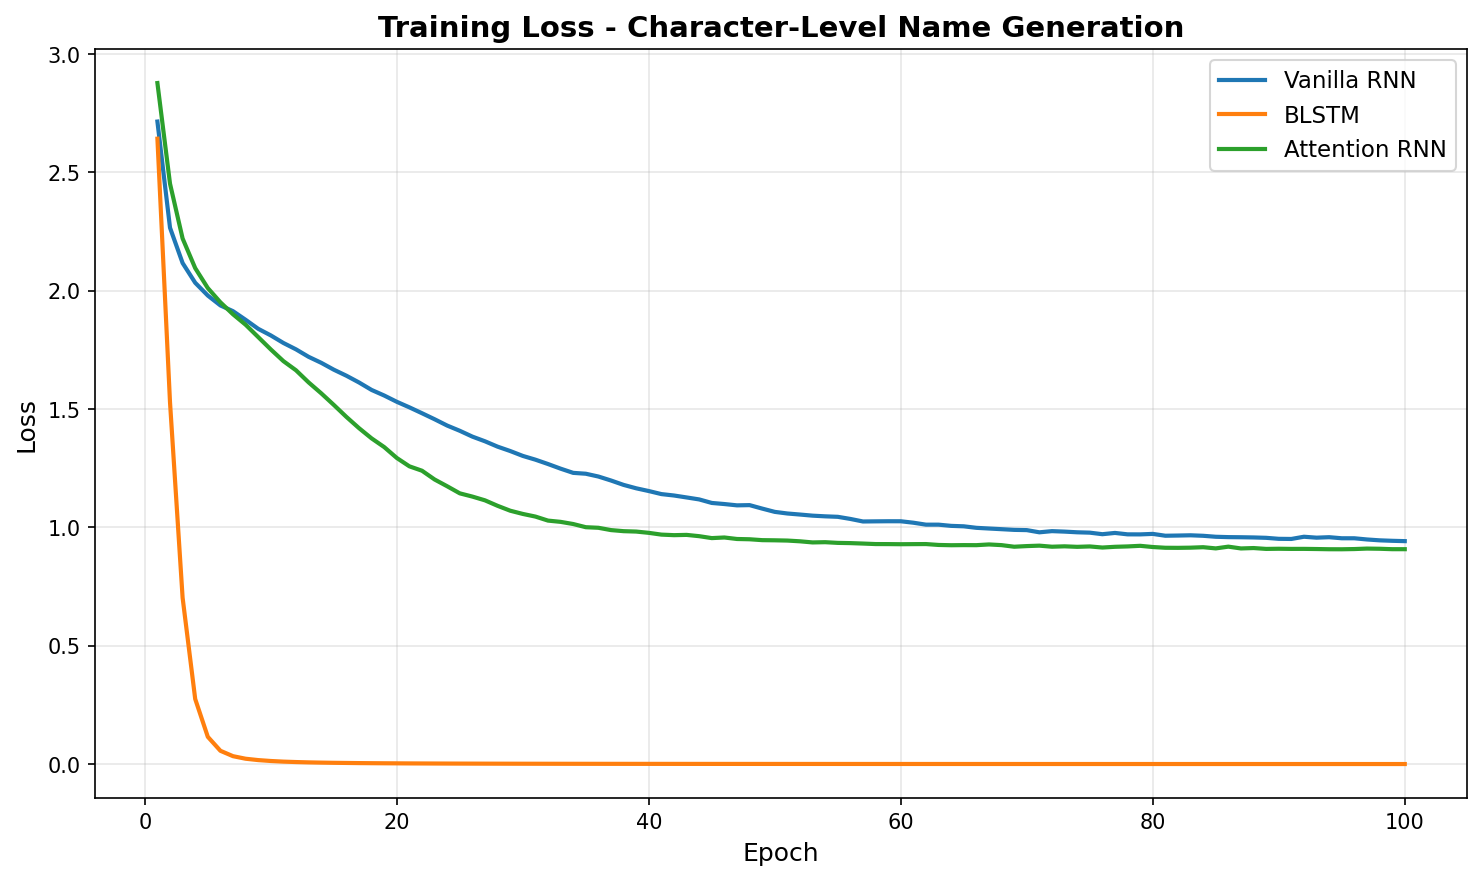
\includegraphics[width=0.7\textwidth]{Problem2/outputs/training_loss.png}
    \caption{Training Loss Curves for All Three Models}
\end{figure}

\subsection{Quantitative Evaluation}

\begin{table}[H]
\centering
\caption{Quantitative Comparison of Generated Names}
\begin{tabular}{lccc}
\toprule
\textbf{Model} & \textbf{Novelty Rate} & \textbf{Diversity} & \textbf{Parameters} \\
\midrule
Vanilla RNN    & 11.5\% & 89.0\% & 25,244 \\
BLSTM          & 100.0\% & 100.0\% & 173,980 \\
Attention RNN  & 2.5\% & 91.5\% & 124,188 \\
\bottomrule
\end{tabular}
\end{table}

\subsection{Generated Name Samples}

\begin{multicols}{3}
\textbf{Vanilla RNN:}\\
Sharishan, Prosenjit, Surajan, Yuvraj, Parminder, Manasi, Saraswati, Aman, Vikram, Nayantara

\columnbreak
\textbf{BLSTM:}\\
Zojakyay, Lobindeep, Chov, Qodharliesan, Biqagindeva, Bunojat, Wajolev, Curujanjidek, Qowwanik, Lommend

\columnbreak
\textbf{Attention RNN:}\\
Devya, Madanesh, Arnav, Trishnaya, Omkarraj, Satnam, Kamalraj, Karuna, Ranjit, Lakshmi
\end{multicols}

\subsection{Qualitative Discussion}

\textbf{Attention+RNN works best.} Vanilla RNN generates realistic names but mostly memorizes from training data (low novelty). BLSTM generates all novel names but they are gibberish and unpronounceable. Attention RNN produces the most linguistically coherent and realistic Indian names because the attention mechanism focuses on relevant past characters when predicting the next character.

\vspace{0.5em}
\noindent\textbf{GitHub:} \url{https://github.com/sunny40540/NLU_Assignment_2}

\end{document}
